\documentclass[english, 9pt, aspectratio=169]{beamer}
\usepackage[utf8]{inputenc}
\usepackage[T1]{fontenc}
\usepackage{lmodern}
\usepackage{babel}
\usetheme{EastLansing}

\usepackage{multicol}

\usepackage{amsmath}
\usepackage{amsfonts}
\usepackage{amssymb}
\usepackage{amsthm}

%\AtBeginSection[]{
%	\begin{frame}
%		\frametitle{Plan}
%		\begin{multicols}{2}
%		\tableofcontents[currentsection]
%		\end{multicols}
%	\end{frame}
%}

%\AtBeginSubsection[]{
%	\begin{frame}
%		\frametitle{Plan}
%		\begin{multicols}{2}
%		\tableofcontents[currentsubsection]
%		\end{multicols}
%	\end{frame}
%}

\begin{document}
\title[Metro-like carpooling on HOV]{High Occupancy Vehicle Lane and Metro-like Carpooling. A Bottleneck Case Study}
\subtitle{State of study}
\titlegraphic{
\includegraphics[width=14cm]{./images/lvmt_enpc_ipp_univlyon2_laet.png}}

\author[MB, NC and GM]{Martin Briand$^{a}$, Nicolas Coulombel$^{b}$, Guillaume Monchambert$^{c}$}
\institute[LVMT, LVMT and LAET]{\small $^{a}$Martin’s affiliation + email --> corresponding author\\
\small $^{b}$Nicolas’ affiliation + email\\
\small $^{c}$Université Lyon 2, LAET}
\date{2025}
\subject{Transportation Economics} %useless only in pdf properties…
\setbeamercovered{invisible}
\setbeamertemplate{navigation symbols}{}
\begin{frame}[plain]
\titlepage
\end{frame}

\begin{frame}{Setup}{Congestion Technology}
    \begin{multicols}{2}
    \begin{itemize}
        \item 3 modes:
        \begin{itemize}
            \item Solo-drivers (subscript $s$)
            \item Carpooling drivers (subscript $d$) taking all passengers waiting at the carpooling station, if any, up to the capacity of the vehicle
            \item Carpooling passengers (subscript $p$) waiting at station for a driver
        \end{itemize}

        \item Road with fixed capacity $s$ shared between reserved capacity $\varphi s$ and capacity for solo-drivers $(1-\varphi)s$ (with $0 \leq \varphi \leq 1$).

        \item Max $M$ passenger per vehicle.

        \item 3 bottlenecks with vertical queue:
        \begin{itemize}
            \item Right before downstream station for solo-drivers (capacity $(1-\varphi)s$)
            \item Right before downstream station for carpooling vehicles (capacity $\varphi s$)
            \item At upstream station for passengers with variable capacity $Mr_d(t)$ where $r_d(t)$ is the rate of carpooling drivers proposing their seats.
        \end{itemize}
    \end{itemize}

    \end{multicols}

    \begin{center}
            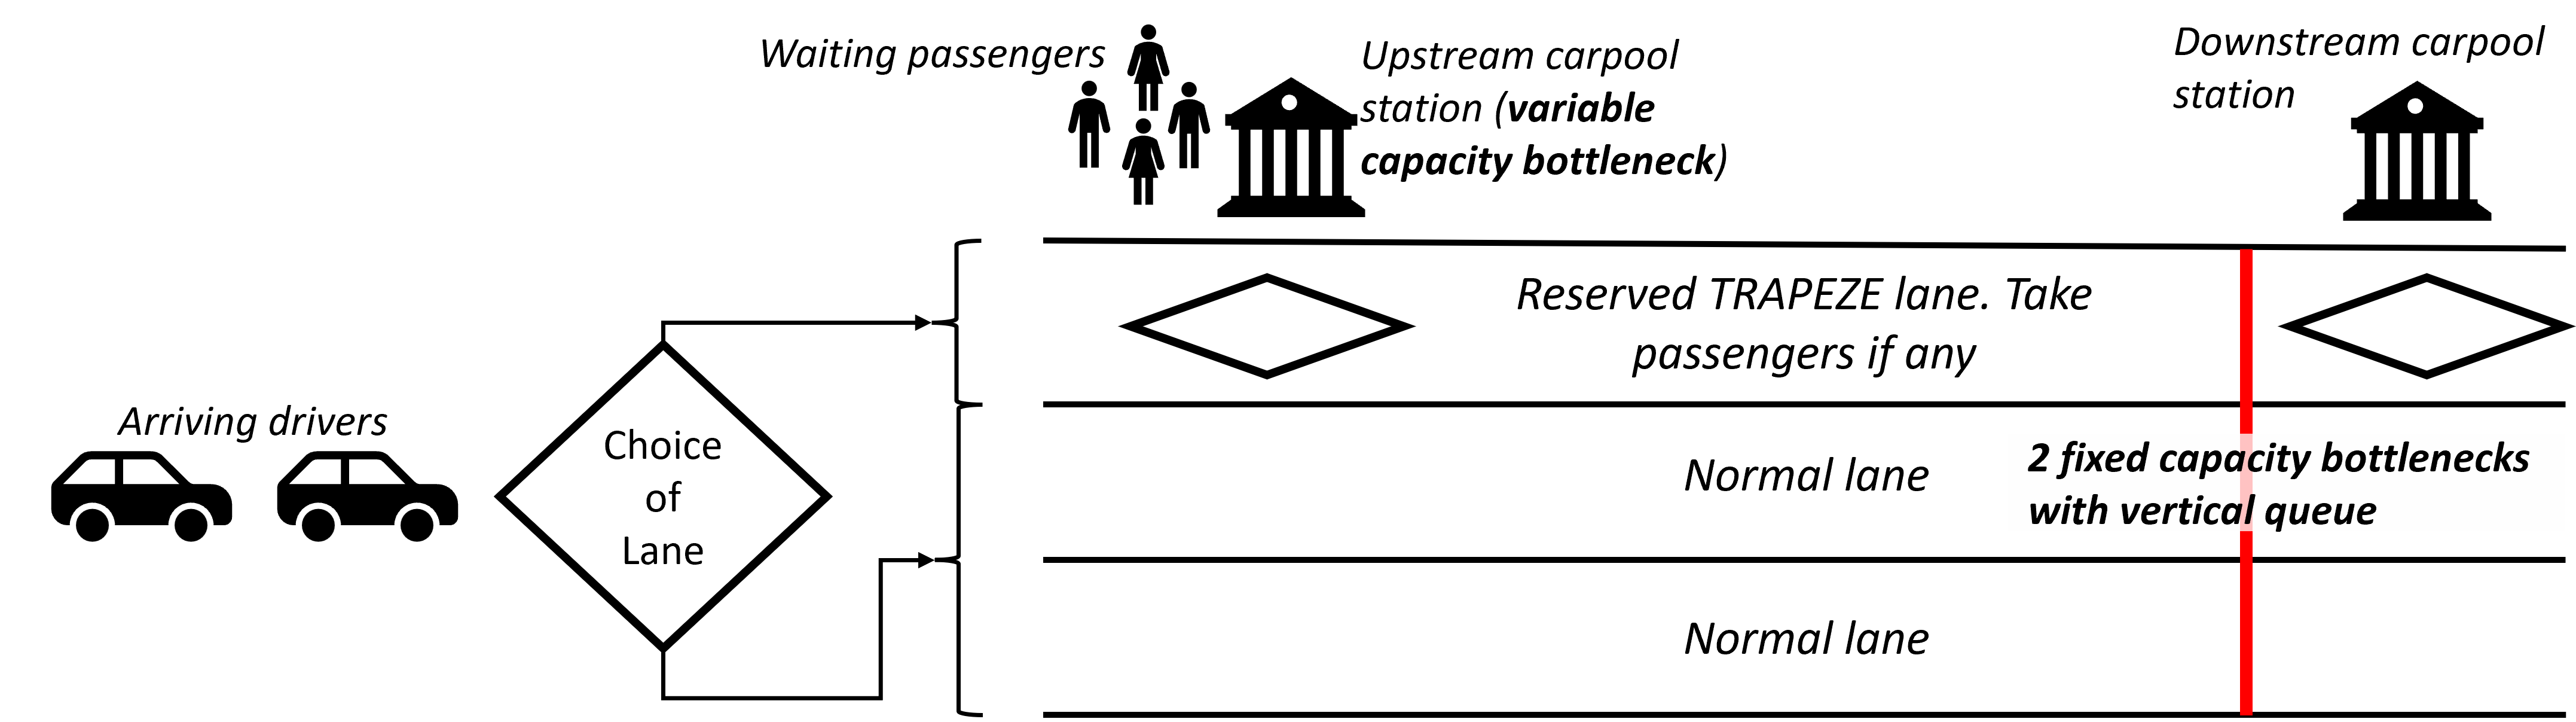
\includegraphics[trim=0cm 0cm 0cm 0cm, clip, width=0.70\textwidth]{images/metro_like_carpool_hov_schema.png}

    \end{center}
\end{frame}

\begin{frame}{Setup}{Demand}
\begin{multicols}{2}
\begin{itemize}
    \item $N$ commuters
    \item Classical bottleneck values of time $\alpha$, $\beta$ and $\gamma$.
    \item Common desired arrival time $t^*$
    \item Environmental costs per car $E$
    \item Car operation costs $f$
    \item Carpooling driver inconvenience cost $\overline{\Delta _d}$
    \item Distributed carpooling passenger inconvenience cost $\Delta _p$. $\Delta _p^{\text{min}} \leq \Delta _p \leq \Delta _p^{\text{max}}$. Distributed according to cumulative distribution function $F$ which is continuous, differentiable and strictly increasing.
    \item Payments for using the carpooling service $\rho _p (t)$ for passengers, and $\rho _d(t)$ for drivers.
\end{itemize}
\end{multicols}

\vfill
\hrulefill
\vfill

\begin{columns}
\begin{column}{.5\textwidth}
Cost experienced by a driver with given $\Delta _p$ value according to her chosen mode:
\begin{equation*}
    \left\{
    \begin{array}{l}
        c_s(t) = \text{tt}_s(t) + \text{sched}_s(t) + f\\
        c_d(t) = \text{tt}_d(t) + \text{sched}_d(t) + f + \overline{\Delta _d} + \rho _d (t)\\
        c_p(t) = \text{tt}_p(t) + \text{sched}_p(t) + \Delta _p + \rho _p (t)
    \end{array}
    \right.
\end{equation*}
\end{column}
\begin{column}{.5\textwidth}

And her contribution to social cost: \alert{j'ai des doutes sur la contribution au coût social. Il semble manquer les externalités proudites sur les autres usagers du botteneck.}
\begin{equation*}
    \left\{
    \begin{array}{l}
        sc_s(t) = c_s(t) + E\\
        sc_d(t) = c_d(t) + E - \rho _d (t)\\
        sc_p(t) = c_p(t) - \rho _p(t)
    \end{array}
    \right.
\end{equation*}
    
\end{column}

\end{columns}
    
\end{frame}


\begin{frame}{Describing equilibria for time-independent payments}{Case $\varphi = 0$}

\begin{itemize}
    \item Everybody drives solo and nobody carpools $(N_s=N, N_d = N_p = 0)$.
    \item Drivers spread accros time according to classical bottleneck model:
\end{itemize}

\vfill
\hrulefill
\vfill

\begin{columns}

\begin{column}{.5\textwidth}
Departure rate:
\begin{equation*}
\label{eq_rs}
r_s(t) = \left\{
\begin{array}{lr}
    0 & \text{if } t<t_s^0\\
    s\left( 1 + \frac{\beta}{\alpha - \beta} \right) & \text{if } t_s^0 \leq t < \tilde{t}_s\\
    s\left( 1 - \frac{\gamma}{\alpha + \gamma} \right) & \text{if } \tilde{t}_s \leq t \leq t_s^1\\
    0 & \text{if } t_s^1 < t
\end{array}
\right.
\end{equation*}
\end{column}

\begin{column}{.5\textwidth}
where:
\begin{equation*}
\label{eq_ts}
\left\{
\begin{array}{l}
    t_s^0 = t^* - \frac{N_s}{s} \times \frac{\gamma}{\beta + \gamma}\\
    \tilde{t}_s = t^* - \frac{N_s}{s} \times \frac{\beta \gamma}{\alpha(\beta + \gamma)}\\
    t_s^1 = t^* + \frac{N_s}{s} \times \frac{\beta}{\beta + \gamma}
\end{array}
\right.
\end{equation*}
\end{column}
\end{columns}
\end{frame}


\begin{frame}{Describing equilibria for time-independent payments}{Case $\varphi = 1$}

\begin{columns}
\begin{column}{.65\textwidth}

\begin{itemize}
    \item Everybody carpools
    \item Let $\Delta _p^{\text{full}} = F^{-1}\left( \frac{M}{M+1} \right)$. (Beyond a proportion $\frac{M}{M+1}$ of passengers, the capacity of cars is full.)
    \item If $\Delta _p^{\text{full}} < f + \Delta _d + \rho _d - \rho _p$, no equilibrium.
    \item If $\Delta _p^{\text{full}} = f + \Delta _d + \rho _d - \rho _p$. Unique equilibrium: $N_d = \frac{N}{M+1}$ and $N_p = \frac{NM}{M+1}$. Drivers spread in time according to classical bottleneck, and passengers according to $r_p(t) = Mr_d(t)$ (picture 3).
    \item If $\Delta _p^{\text{min}} \geq f + \Delta _d + \rho _d - \rho _p$. Unique equilibrium: $N_d = N$ and $N_p = 0$. Drivers spread in time according to classical bottleneck (picture 1).
    \item Else, there exist a $\Delta _p^{\text{min}} < \Delta _p^{\text{switch}} < \Delta _p^{\text{full}}$ such that $\Delta _p^{\text{switch}} = f + \Delta _d + \rho _d - \rho _p$. We have $N_p = NF(\Delta _p^{\text{switch}})$ passengers and $N_d = N-N_p$ drivers. All drivers have $\Delta _p \geq \Delta _p^{\text{switch}}$ and passengers have $\Delta _p \leq \Delta _p^{\text{switch}}$. Drivers spread in time according to classical bottleneck, and passengers however they want as long as they never queue (picture 2).
\end{itemize}

\end{column}



\begin{column}{.35\textwidth}
\begin{center}
    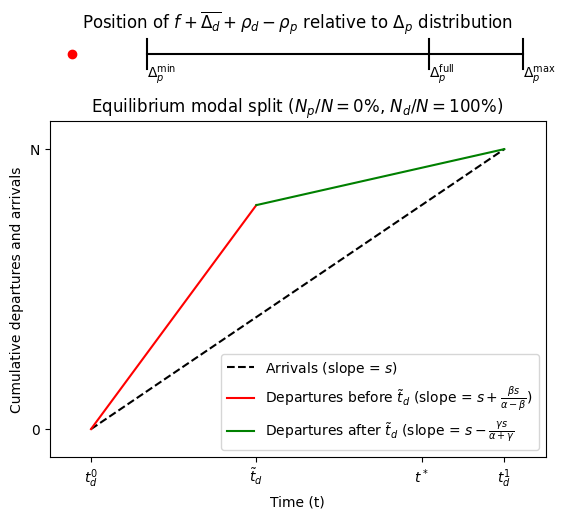
\includegraphics[trim=0cm 0cm 0cm 0cm, clip, width=0.49\textwidth]{images/arrivals1.png}
    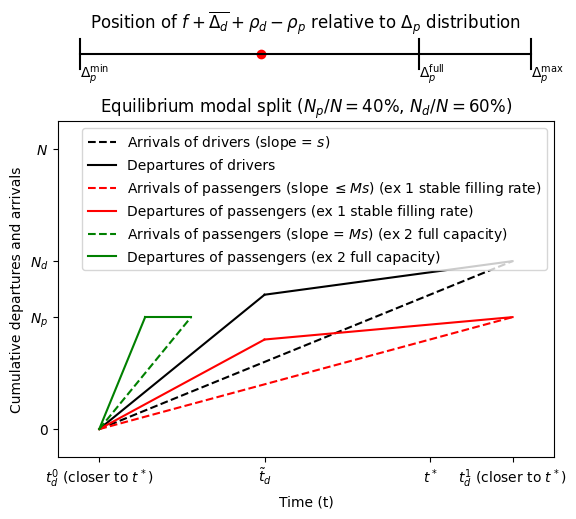
\includegraphics[trim=0cm 0cm 0cm 0cm, clip, width=0.49\textwidth]{images/arrivals2.png}
    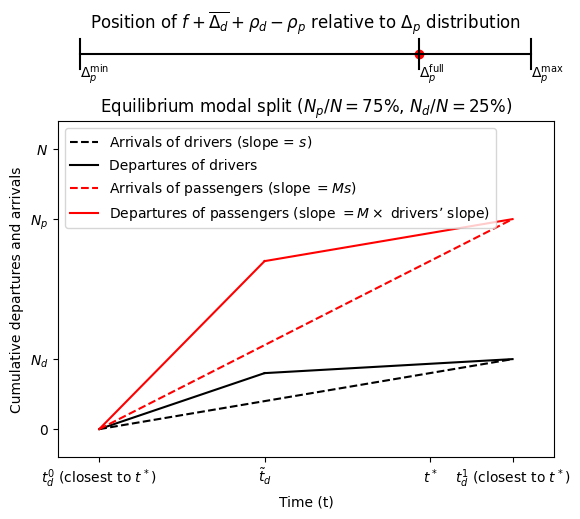
\includegraphics[trim=0cm 0cm 0cm 0cm, clip, width=0.49\textwidth]{images/arrivals3.png}
\end{center}
\end{column}
\end{columns}

    
\end{frame}


\begin{frame}{Describing equilibria for time-independent payments}{Case $0 < \varphi < 1$}

\begin{columns}
\begin{column}{0.65\textwidth}

\begin{itemize}
    \item It is possible to have no equilibrium (area F).
    \item Else, if there is an equilibrium, the equilibrium involves a unique modal split where passengers are clearly identified in the population (the $N_p$ with the lowest $\Delta _p$). As long as car capacity is not reached and that there are some passengers, departure times of passengers is non-unique (area E + area D + line 4), otherwise, it is.
    \item Potential equilibrium is one of the 7 below (equations in paper):
    \begin{itemize}
        \item Everybody drives solo (area A + line 1).
        \item Everybody carpools
        \begin{itemize}
            \item but everybody drives (area C + line 3 + line 2 below C);
            \item and the car capacity of carpooling drivers is reached (line 6);
            \item and the car capacity is not reached while some are passengers (area D + line 4).
        \end{itemize}
        \item Some drive solo and some carpool
        \begin{itemize}
            \item but everybody drives (area B + line 2 below B);
            \item and the car capacity of carpooling drivers is reached (line 5);
            \item and the capacity of car is not reached while some are passengers (area E).
        \end{itemize}
    \end{itemize}
\end{itemize}

\end{column}

\begin{column}{0.35\textwidth}
\begin{center}
    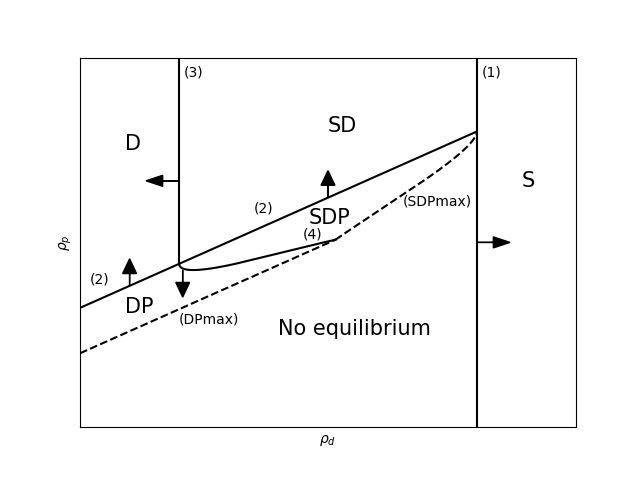
\includegraphics[trim=0cm 0cm 0cm 0cm, clip, width=\textwidth]{images/equilibrium_phase_diagram_trapezoidal_dist.png}

    \small{Arrows show to what area each line belongs to form a certain type of equilibrium (or non-equilibrium for area F).}
\end{center}
\end{column}
\end{columns}

\end{frame}

\begin{frame}{Choosing equilibria for time-independent payments and fixed $0 < \varphi \leq 1$}

\begin{itemize}
    \item For any feasible modal split ($N_i \geq 0$, $i\in \left\{ s,d,p \right\}$, $N_s + N_p + N_d = N$ and $N_p \leq MN_p$, there is a non necessary unique fare policy $(\rho_d, \rho_p)$ such that the feasible modal split is the unique one with equilibria for that fare policy.

    \item Since, for any fare policy with equilibria, social can be expressed as a function of $(N_s, N_p, N_d)$ (independent of the fare policiy). Optimizing social cost can be reduced to choosing the best feasible modal splits. 
\end{itemize}
\end{frame}

\begin{frame}{Next steps}

\begin{itemize}
    \item Describe equilibrium with nice visuals
    \item Optimize social cost for time-independent fare policies and for a fixed $\varphi$.
    \item Optimize social cost for time-independent fare policies and jointly with $\varphi$.
    \item Decentralize congestion with time-dependent fare policies to get almost first-best equilibrium but for fixed $\varphi$.
    \item Decentralize congestion and optimize jointly with $\varphi$.
    \item Could we do it again for a more normal reserved lane less like TRAPEZE?
\end{itemize}

\end{frame}

\begin{frame}{Optimize Social cost for time-independent fare policies and for a fixed $\varphi$}

\begin{center}
    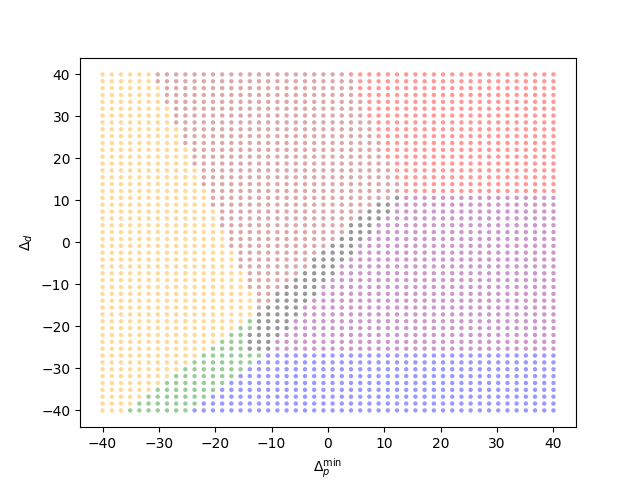
\includegraphics[trim=0cm 0cm 0cm 0cm, clip, width=.6\textwidth]{images/equilibrium_phase_diagram_trig_dist_phi_fixed_N10000.png}

    \small{Phase diagram of optimal for $N = 10^4$}
\end{center}


    
\end{frame}

\begin{frame}{Optimize Social cost for time-independent fare policies and for a fixed $\varphi$ and $N \rightarrow 0$}

\begin{center}
    Graph is still TODO but equations are written in the other project
\end{center}


    
\end{frame}

\begin{frame}{Optimize Social cost for time-independent fare policies and for a fixed $\varphi$ and $N \rightarrow +\infty$}

\begin{center}
    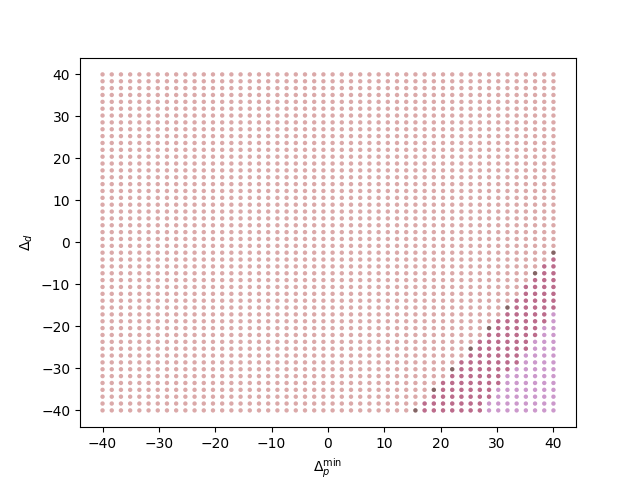
\includegraphics[trim=0cm 0cm 0cm 0cm, clip, width=.6\textwidth]{images/equilibrium_phase_diagram_trig_dist_phi_fixed_N1000000.png}

    \small{Phase diagram of optimal for $N = 10^6$. Case j becomes predominant}.
\end{center}


    
\end{frame}

\begin{frame}{Some examples}

\begin{columns}
\begin{column}{0.8\textwidth}
\begin{itemize}
    \item $\alpha = 2$, $\beta = 1$, $\gamma = 4$, $\delta = 4 / 5$
    \item $s=2000$, $f = 1$, $E = 1$, $\varphi = 0.7$
    \item $\Delta_d = 2$, $\Delta_p^{\text{min}} = -2$, $\Delta_p^{\text{max}} - \Delta_p^{\text{min}} = 15$, $F$ is trig dist ($c=0.7$).
\end{itemize}
What is interesting
\begin{itemize}
    \item A regime change in the middle (interior) (not the case with uniform distribution
    \item Drivers pay despite negative $\Delta_d$
    \item Passengers are paid
    \item Negative profit still
\end{itemize}
\end{column}

\begin{column}{0.2\textwidth}

\begin{center}
    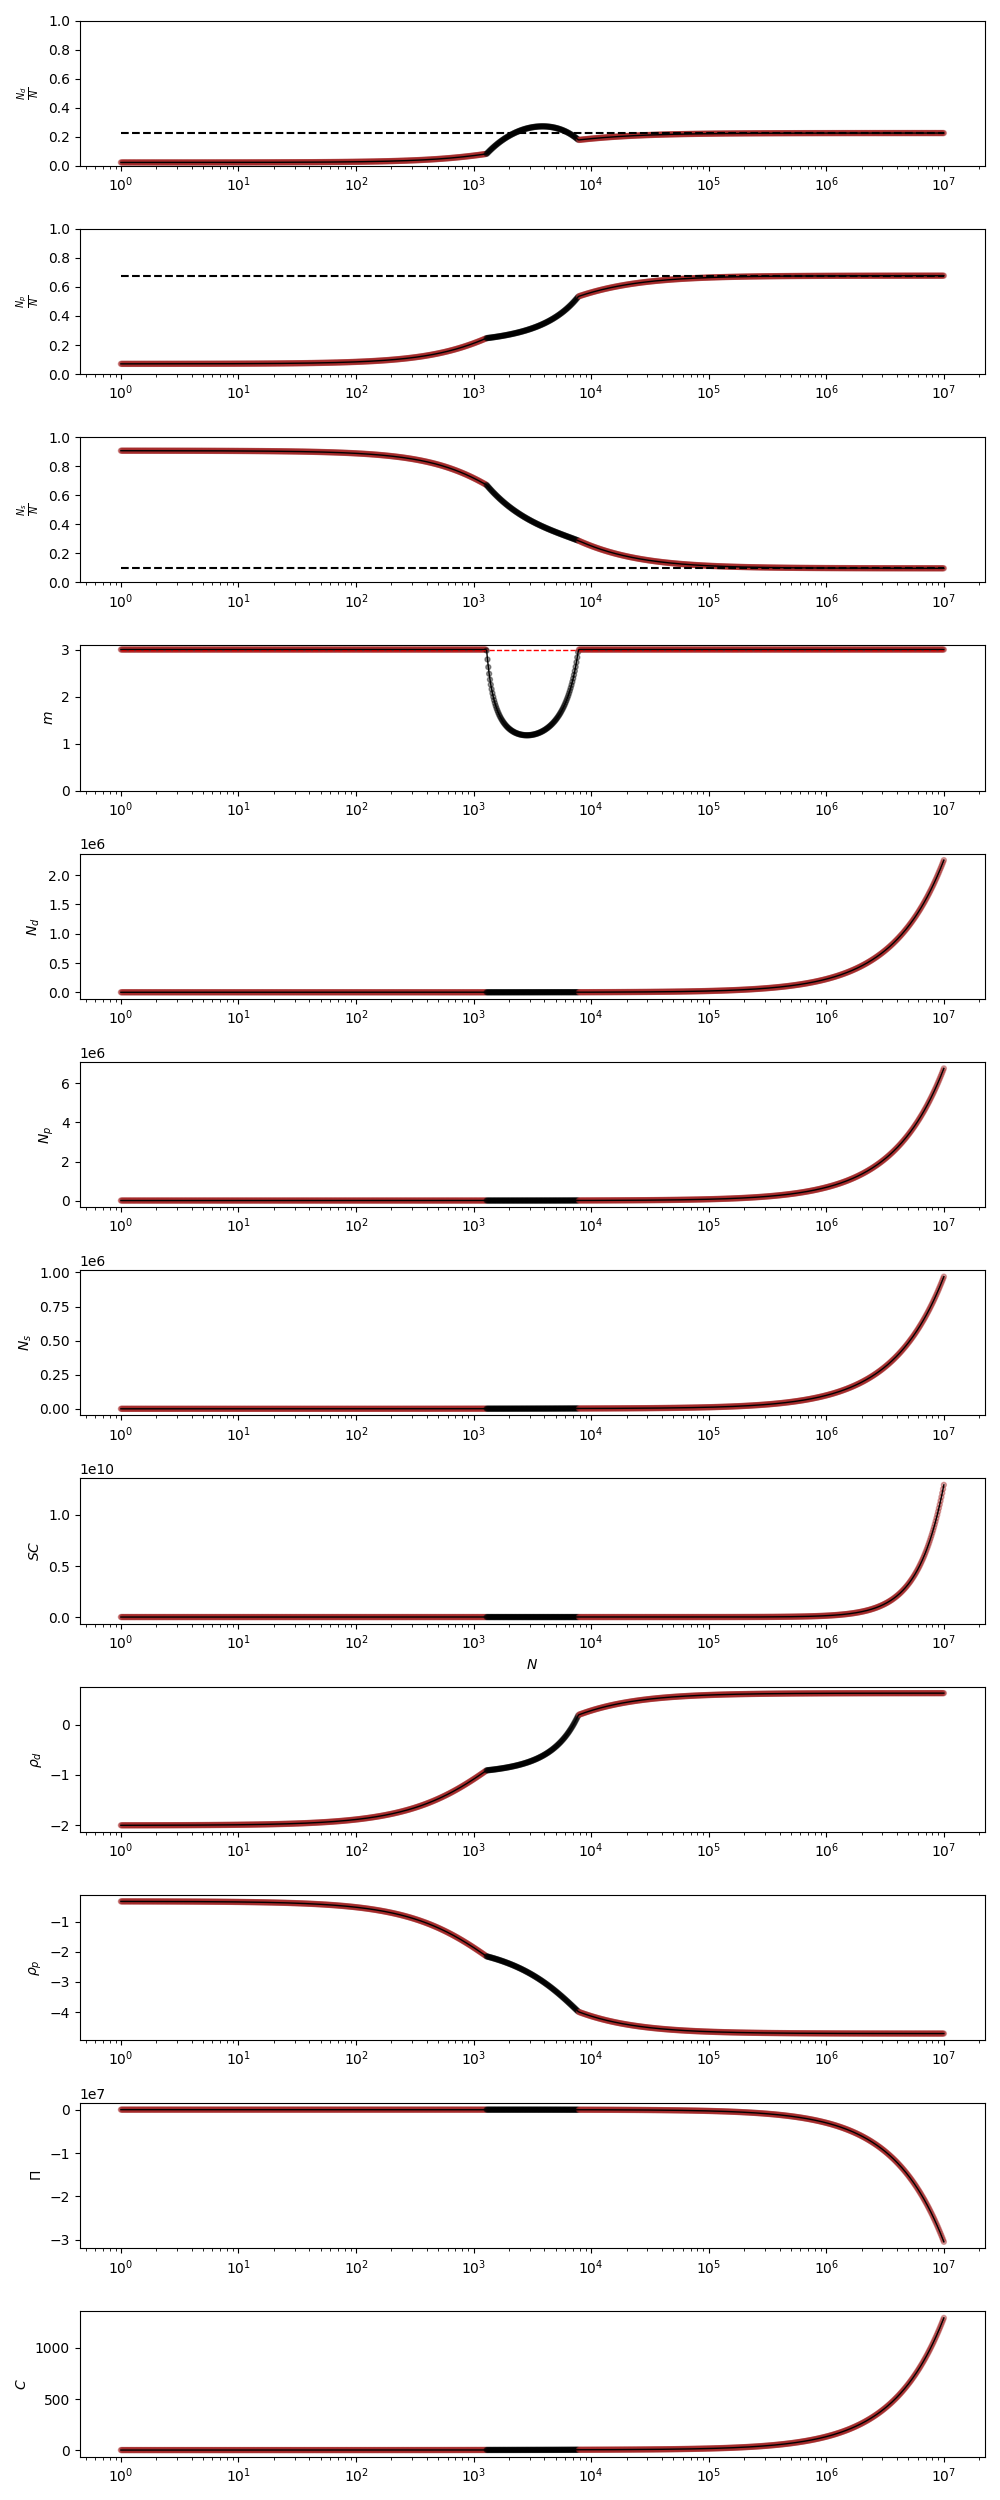
\includegraphics[trim=0cm 0cm 0cm 0cm, clip, width=.9\textwidth]{images/evolution_of_values_phi_fixed_1.png}

    \small{Case 1}.
\end{center}

\end{column}
    
\end{columns}

\begin{center}
    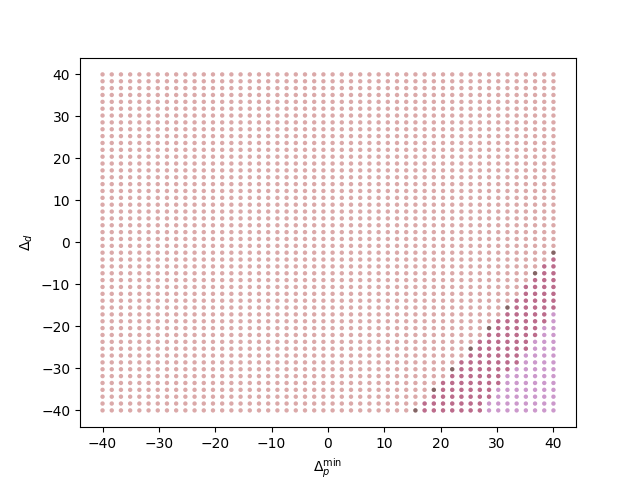
\includegraphics[trim=0cm 0cm 0cm 0cm, clip, width=.6\textwidth]{images/equilibrium_phase_diagram_trig_dist_phi_fixed_N1000000.png}

    \small{Phase diagram of optimal for $N = 10^6$. Case j becomes predominant}.
\end{center}


    
\end{frame}



\begin{frame}{Optimizing for $N \rightarrow 0$}

\begin{center}
    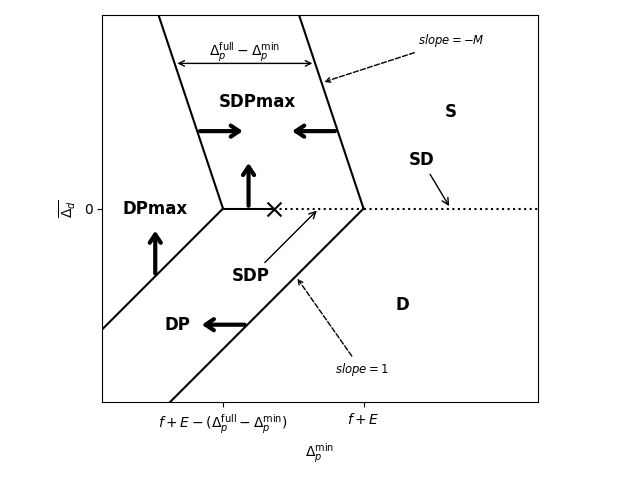
\includegraphics[trim=0cm 0cm 0cm 0cm, clip, width=.6\textwidth]{images/optimal_regime_phase_diagram_Nto0.png}

    \small{Phase diagram of optimal as $N \rightarrow 0$}
\end{center}
    
\end{frame}


\end{document}